\chapter{Group theory}
\section{The bare minimum}
\subsection{Symmetry elements and symmetry operations}
\begin{defi}[Symmetry operations]
A \textbf{symmetry operation} is an operation about a \textbf{symmetry element} 
that leaves the object (molecule) \textit{apparently} unchanged. 
The actual particles may well have changed places but 
the important thing is that we can't tell. 
\end{defi}
\begin{defi}[Symmetry elements]
A \textbf{symmetry element} is said to \textit{generate} symmetry operations, for example, an axis of rotation can generate rotation. 
\end{defi}
There are only 5 types of symmetry operations and the symmetry elements that 
generate them: 
\begin{table}[H]
\centering
\begin{tabular}{l|l}
Operation & Element\\
\hline
$E$, the \textbf{identity}& The object itself\\
$C_n$, the \textbf{$\boldsymbol{n}$-fold rotation}& The axis of symmetry\\
$\sigma$, the \textbf{reflection}& The mirror plane\\
$i$, the \textbf{inversion}& The centre of symmetry\\
$S_n$, the \textbf{$\boldsymbol{n}$-fold improper rotation}& The axis of improper rotation
\end{tabular}
\caption{The 5 symmetry operations and their generating elements.}
\end{table}
Some important nomenclature:
\begin{enumerate}
	\item $C_n$
	\begin{enumerate}
	 	\item The element with highest $n$ is called the \textbf{principle axis}.
	 	\item For $n>2$, an axis can generate two directions of rotation, for example, we have $2C_4$ belonging to the $D_{4h}$ group. 
	 \end{enumerate}
	 \item $\sigma$
	 \begin{enumerate}
	 	\item When the element (mirror plane) includes the principle axis, it's called a \textbf{vertical plane}, $\sigma_v$.
	 	\item When the element is perpendicular to the principle axis, it's called a \textbf{horizontal plane}, $\sigma_h$.
	 	\item A special type of vertical planes is when it bisects the angle between two $C_2$ axes. It's then called a \textbf{dihedral plane}, $\sigma_d$.
	 \end{enumerate}
\end{enumerate}
\subsection{Point groups}
We use a symmetry flow chart to determine the point group a molecule belongs to:
\begin{figure}[ht]
	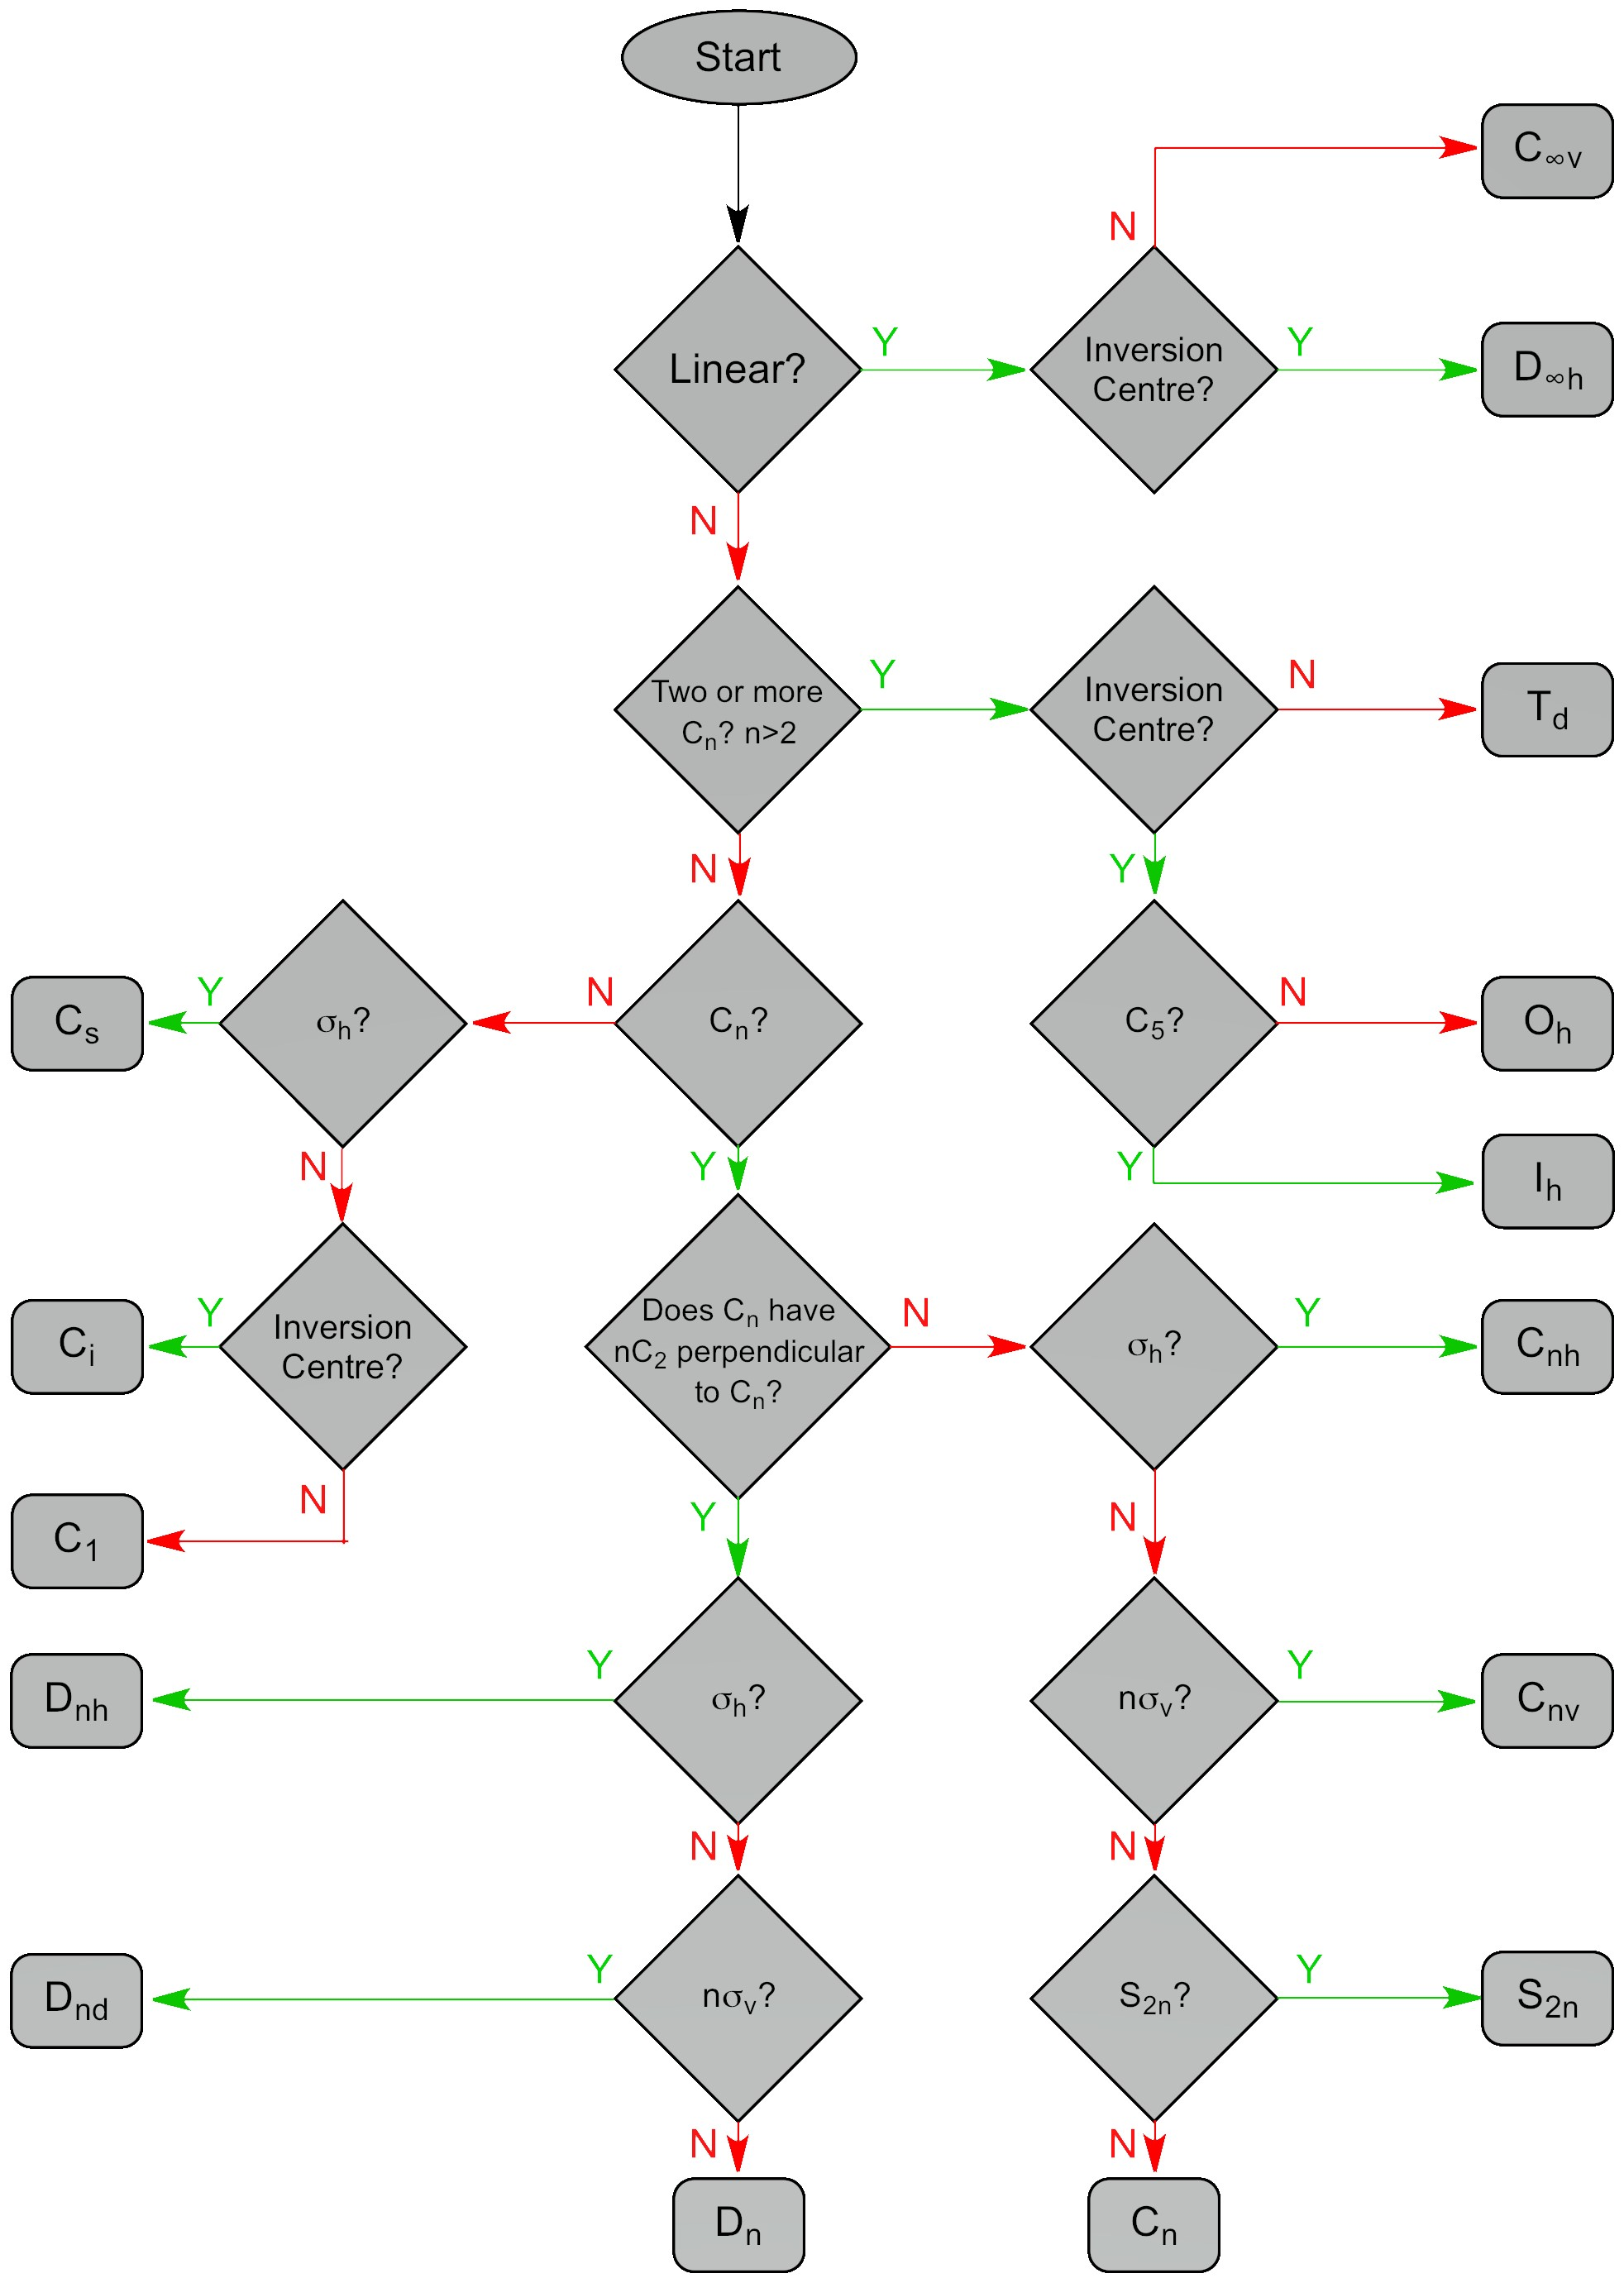
\includegraphics[width=11cm]{symflow}
	\centering
	\caption{Flowchart used to determine point groups.}
	\label{fig:symflow}
\end{figure}
Example molecules can be found in \cite{wiki_pointgroup}. 
\subsection{Representations}
\begin{defi}[Matrix representations]
A \textbf{matrix representation} is a set of \textbf{matrix representatives}, 
which presents the effect of a \textit{symmetry operation} on a molecule, 
in an \textbf{arbitrarily chosen basis}. 
\end{defi}
The choice of basis, although technically arbitrary, is usually just vectors along 
the bonds pointing from the central atom or the atomic orbitals, 
amongst other conventions for other applications. \par
For any arbitrarily chosen basis, a matrix representation can be generated. 
We can use the results from the great and little orthogonality theorems 
(see 5.10-5.11 of \cite{atkinsqm}) to \textit{reduce} a representation to 
see how many of each irreducible representation is present in the direct sum. 
Due to a theorem in group theory that states that the character (trace) of a 
representative is invariant under a change of basis (a familiarity transform), 
we can work with characters instead of matrices. 
An essential theorem on reducing representations 
(more accurately, charaters of representations) is as follows:
\begin{thrm}[Reducing representations]
The number of times an irreducible representation occurs in the reducible representation is given by
\begin{equation}
a(I)=\frac{1}{h}\sum_{\text{all classes}}\chi(R)\chi(I)N
\end{equation}
where
\begin{equation*}
\begin{aligned}
h&=\text{order of the group}\\
\chi(R)&=\text{character of the reducible representation}\\
\chi(I)&=\text{character of the irreducible representation}\\
N&=\text{number of symmetry operations in the class}
\end{aligned}
\end{equation*}
\end{thrm}
\section{Mathematical formulation}
\subsection{Notations}
See the following table for the notation we will employ: 
\begin{table}[H]
\centering
\begin{tabular}{l|l}
Meaning & Notation\\
\hline
Basis (a row vector)&$\boldsymbol{f}=(f_1,f_2,\cdots,f_d)$\\
Symmetry operations&$R,\ S,\ T,\cdots$\\
Representation of operations&$\boldsymbol{D}(R)$\\
Operation on basis&$R\boldsymbol{f}\equiv\boldsymbol{f}\boldsymbol{D}(R)$\\
Character of representation&$\chi(R)\equiv\text{tr}\bvec{D}(R)$
\end{tabular}
\caption{Notations used in group theory.}
\end{table}
\subsection{Basic theorems}
We now go on to establish some fundamental lemmas to build on later.
\begin{lemma}[Representation of group multiplication]
If $RS=T$, then $\boldsymbol{D}(R)\boldsymbol{D}(S)=\boldsymbol{D}(T)$.
\end{lemma}
\begin{proof}
\begin{equation}
\begin{aligned}
&RS\boldsymbol{f}=R[\boldsymbol{f}\boldsymbol{D}(S)]=(R\boldsymbol{f})\boldsymbol{D}(S)=\boldsymbol{f}\boldsymbol{D}(R)\boldsymbol{D}(S)=T\boldsymbol{f}=\boldsymbol{f}\boldsymbol{D}(T)\\
&\imp \boldsymbol{D}(R)\boldsymbol{D}(S)=\boldsymbol{D}(T)
\end{aligned}
\end{equation}
\end{proof}
\begin{lemma}[Representation of the inverse of operation]
The representative of the inverse of an operation is 
the inverse of the representative: 
\begin{equation}
\bvec{D}(R^{-1})=\bvec{D}(R)^{-1}. 
\end{equation}
\end{lemma}
\begin{proof}
Because we know that
\begin{equation}
RR^{-1}=E
\end{equation}
so
\begin{equation}
\bvec{D}(R)\bvec{D}(R^{-1})=\bvec{D}(E)=\bvec{I}
\end{equation}
therefore we can identify $\bvec{D}(R^{-1})$ with $\bvec{D}(R)^{-1}$.
\end{proof}
Oftentimes we would like to change the basis of a representation to simplify it, 
\ie to reduce it. We also call a change of basis a 
\textbf{similarity transformation}. An example could be the NH$_3$ molecule, where 
we originally choose a basis set of the three $s$-orbitals. But, as it will turn 
out, this is not the basis for the irreducible representation, and to find it we 
need to compute the symmetry-adapted bases of the molecule (\hl{update link}). 
Now say we have the new basis, given by 
\begin{equation*}
\begin{aligned}
s_N&=s_N\\
s_1&=s_A+s_B+s_C\\
s_2&=2s_A-s_B-s_C\\
s_3&=s_B-s_C
\end{aligned}
\end{equation*}
or, in matrix notation
\begin{equation}
\bvec{f}'\equiv\bvec{f}
\underbrace{
\begin{bmatrix}
1 &0 &0 &0\\
0 &1 &2 &0\\
0 &1 &-1& 1\\
0 &1 &-1& -1
\end{bmatrix}}_{\equiv\bvec{c}}
\end{equation}
the question is then, how to we find the representative, $\bvec{D}(R)$ in this new basis?
\begin{thrm}[Similarity transformation]
We say that two representations are \textbf{similar} if the representatives for 
the two bases are related by the \textbf{similarity transformation}:
\begin{equation}
\bvec{D}(R)=\bvec{c}\bvec{D}'(R)\bvec{c}^{-1}\ \leftrightarrow\ \bvec{D}'(R)=\bvec{c}^{-1}\bvec{D}(R)\bvec{c}.
\end{equation}
\end{thrm}
\begin{proof}
\begin{equation}
\begin{aligned}
R\bvec{f}'&=\bvec{f}'\bvec{D}'(R)\\
R\bvec{fc}&=\bvec{fcD}'(R)\\
R\bvec{f}&=\bvec{fcD}'(R)\bvec{c}^{-1}=\bvec{fD}(R)
\end{aligned}
\end{equation}
The result is immediately implied. 
\end{proof}
We introduce a lemma from linear algebra:
\begin{lemma}[Trace is invariant under cyclic permutation]
\begin{equation}
\text{tr}\bvec{ABC}=\text{tr}\bvec{BCA}=\text{tr}\bvec{CAB}.
\end{equation}
\end{lemma}
\begin{proof}
\begin{equation}
\text{tr}\bvec{ABC}=(ABC)_{ii}=A_{ik}B_{jk}C_{ki},
\end{equation}
where we have used the Einstein summation convention. Under cyclic permutation, 
the subscript continue to match, hence giving invariant trace. 
\end{proof}
\begin{thrm}[Character is invariant under similarity transform]
\label{charinv}
\begin{equation}
\chi(R)=\chi'(R).
\end{equation}
\end{thrm}
\begin{proof}
\begin{equation}
\chi(R)=\text{tr}\bvec{cD}'(R)\bvec{c}^{-1}=\text{tr}\bvec{D}'(R)=\chi'(R).
\end{equation}
\end{proof}
We need to categorise operatioons into classes, which is defined by
\begin{defi}[Classes]
Operations $R$ and $R'$ are said to be in the same class, 
or are \textit{conjugate}, if they are related as follows:
\begin{equation}
R'=S^{-1}RS, 
\end{equation}
which is to say, they are the same \textit{kind} of operation but performed 
about symmetry elements that are \textit{related by a symmetry operation}. 
\end{defi}
\begin{thrm}[Operations in the same class have the same character]
\begin{equation}
\chi(R')=\chi(R).
\end{equation}
\end{thrm}
\begin{proof}
\begin{equation}
\chi(R')=\text{tr}\bvec{D}(R')=\text{tr}\bvec{D}^{-1}(S)\bvec{D}(R)\bvec{D}(S)=\text{tr}\bvec{D}(R)=\chi(R).
\end{equation}
\end{proof}
\subsection{Irreps and orthogonality theorems}
We return to the example of NH$_3$, which belongs to the group $C_{3v}$. 
In the basis of $(s_N,s_1,s_2,s_3)$, all the representatives of 
the group operations all have two diagonal $1$'s at the top left. 
The remaining matrices are
\begin{table}[H]
\centering
\begin{tabular}{l l l}
$\bvec{D}(E)$&$\bvec{D}(C_3^+)$&$\bvec{D}(C_3^-)$\\
$
\begin{bmatrix}
1&0\\
0&1
\end{bmatrix}
$&
$\begin{bmatrix}
-1/2&-1/2\\
1/1&-1/2
\end{bmatrix}$&
$\begin{bmatrix}
-1/2&1/2\\
-1/2&-1/2
\end{bmatrix}$\\
$\bvec{D}(\sigma_v)$&$\bvec{D}(\sigma'_v)$&$\bvec{D}(\sigma''_v)$\\
$\begin{bmatrix}
1&0\\
0&-1
\end{bmatrix}$&
$\begin{bmatrix}
-1/2&1/2\\
3/2&1/2
\end{bmatrix}$&
$\begin{bmatrix}
-1/2&-1/2\\
-3/2&1/2
\end{bmatrix}$
\end{tabular}
\end{table}
We can write this as 
\begin{equation}
\bvec{D}^{(4)}=\bvec{D}^{(1)}\oplus \bvec{D}^{(1)}\oplus \bvec{D}^{(2)}
\end{equation}
All three of them are \textbf{irreducible representations} of group $C_{3v}$. 
We know that $\bvec{D}^{(2)}$ is an irreducible representation because the set 
of two by two matrices are not simultaneously diagonalisable, \ie they do not 
commute. \hl{todo: udpate link to relevant qm section}\par 
The basis for the first two $\bvec{D}^{(1)}$'s are $s_N$ and $s_1$ respectively, 
we call them
\begin{defi}[Unfaithful representation]
An \textbf{unfaithful representation} of a group is a trivial one by one matrix 
with $1$ as the sole element. 
\end{defi}
We can see that the characters for them are $(1,1,1,1,1,1)$, which means they 
belong to the $A_1$ symmetry species. The remaining irreps have characters 
$(2,-1,-1,0,0,0)$, which put them under the species $E$. $A_1$ and $E$ are also 
called $\Gamma^{(1)}$ and $\Gamma^{(3)}$ respectively. \par
Now we proceed to introduce the two very important orthogonality theorems:
\begin{thrm}[The great orthogonality theorem (GOT)]
For a group of order $h$, let $D^{(\ell)}(R)$ be the representative of the 
operation $R$ in a $d_{\ell}$-dimensional irrep of symmetry species $\Gamma^{(\ell)}$ of 
the group, then
\begin{equation}
\sum_R D_{ij}^{(\ell)}(R)^*D_{i'j'}^{(\ell')}(R)=\frac{h}{d_{\ell}}\delta_{\ell\ell'}\delta_{ii'}\delta_{jj'}.
\end{equation}
\end{thrm}
This is really a postulate at this point because we will not prove it. 
For most practical purposes though we just need the 
\begin{thrm}[The little orthogonality theorem (LOT)]
\begin{equation}
\sum_R\chi^{(\ell)}(R)^*\chi^{(\ell')}(R)=h\delta_{\ell\ell'}.
\end{equation}
\end{thrm}
\begin{proof}
We set $j=i$ and $j'=i'$, and sum over diagonal entries since we need the trace:
\begin{equation}
\begin{aligned}
\sum_{i,i'}\sum_R D_{ii}^{(\ell)}(R)^*D_{i'i'}^{(\ell')}(R)&=\sum_R\chi^{\ell}(R)^*\chi^{(\ell')}(R)\\
&=\sum_{i,i'}\frac{h}{d_{\ell}}\delta_{\ell\ell'}\delta_{ii'}\delta_{jj'}\\
&=h\delta_{\ell\ell'}, 
\end{aligned}
\end{equation}
we used the fact that the representation is of dimension $d_{\ell}$.
\end{proof}
We can simplify the theorem further by writing 
\begin{equation}
\sum_cg(c)\chi^{(\ell)}(c)^*\chi^{(\ell')}(c)=h\delta_{\ell\ell'},
\end{equation}
where $c$ is the class and $g(c)$ is the number of operations in the class. 
Setting $\ell=\ell'$ we have
\begin{equation}
\sum_cg(c)|\chi^{(\ell)}(c)|^2=h.
\end{equation}
This says that \textit{the sum of squares of the characters of any irreps of a group is equal to the order of the group}. \par
Recasting this in a vector, we can say that $\{g(c)\}^{1/2}\chi_c^{(\ell)}$ is 
a component $v_c^{(\ell)}$ of the vector $\bvec{v}^{(\ell)}$, whose components are 
distinguished by the subscript $c$. The LOT can now be written as
\begin{equation}
\bvec{v}^{(\ell)*}\cdot\bvec{v}^{(\ell')}=h\delta_{\ell\ell'}.
\end{equation}
This is saying that the two vectors are orthogonal unless $\ell'=\ell$. 
However, the number of orthogonal vectors cannot exceed the dimension of the 
space (can be far less if some of them are linearly dependent). Another analysis 
from the GOT tells that the two are actually equal. So we reach 
\begin{thrm}[Restriction 1]
The number of symmetry species is equal to the number of classes.
\end{thrm}
This analysis can be extended to GOT, with $D_{ij}^{(\ell)}(R)$ being the $R$-th 
component of a vector $\bvec{v}$ identified by three indices $\ell$, $i$ and $j$: 
\begin{equation}
\bvec{v}^{(\ell,i,j)*}\cdot\bvec{v}^{(\ell',i',j')}=\frac{h}{d_{\ell}}\delta_{\ell\ell'}\delta_{ii'}\delta_{jj'}.
\end{equation}
As the component index is $R$, we know the vectors are $h$-dimensional. Also, for 
a given $\ell$ (species/irrep), there are $d_{\ell}^2$ vectors. Therefore, 
a similar argument as the one above concludes that 
\begin{equation}
\sum_{\ell}d_{\ell}^2\leq h.
\end{equation}
We assert that the equality in fact holds, so
\begin{thrm}[Restriction 2]
\begin{equation}
\sum_{\ell}d_{\ell}^2=h.
\end{equation}
\end{thrm}
\subsection{Reducing representation}
We wish to find a suitable similarity transform that enables us to write a 
representation as a direct sum of irreps:
\begin{equation}
\bvec{D}(R)\leftrightarrow \bvec{D}'(R)=\bvec{D}^{(\Gamma^{(1)})}(R)\oplus\bvec{D}^{(\Gamma^{(2)})}(R)\oplus\cdots
\end{equation}
We introduce the notation
\begin{equation}
\Gamma=\sum_{\ell}a_{\ell}\Gamma^{(\ell)}, 
\end{equation}
where the sum is really a direct sum and multiplication is repeated direct sums 
and $a_{\ell}$ is how many times the irrep appears in the direct sum. \par
We realise that we need not necessarily find the similarity transform to find 
the coefficient $a_{\ell}$, because we can invoke \Cref{charinv}, and we can say 
\begin{equation}
\chi(R)=\chi'(R)=\sum_{\ell}a_{\ell}\chi^{(\ell)}(R).
\end{equation}
Now, determining the coefficient is within reach. Let's multiply both sides by 
$\chi^{(\ell')}(R)^*$ nad sum over all elements of the group: 
\begin{equation}
\begin{aligned}
\sum_R\chi^{(\ell')}(R)^*\chi(R)&=\sum_R\sum_{\ell}a_{\ell}\chi^{(\ell')}(R)^*\chi^{(\ell)}(R)\\
&=h\sum_{\ell}a_{\ell}\delta_{\ell\ell'}=ha_{\ell'}.
\end{aligned}
\end{equation}
Therefore
\begin{thrm}[Reduction of representations]
\begin{equation}
a_{\ell}=\frac{1}{h}\sum_{R}\chi^{(\ell)}(R)^*\chi(R).
\end{equation}
In terms of classes, 
\begin{equation}
a_{\ell}=\frac{1}{h}\sum_c g(c)\chi^{(\ell)}(c)^*\chi(c).
\end{equation}
\end{thrm}
\subsection{Symmetry-adapted bases}
After establishing the coefficients we may wish to find out what the similarity 
transformation was (which was not necessary if we just wanted to know the 
coeefficients), in other words, we can find out the basis of the new 
representation. The basis is called \textbf{symmetry-adapted basis} and the basis 
functions are called \textbf{symmetry-adapted linear combinations} (SALC). \par
We need to define
\begin{defi}[Projection operator]
The \textbf{projection operator} is defined as 
\begin{equation}
P_{ij}^{(\ell)}=\frac{d_{\ell}}{h}\sum_RD_{ij}^{(\ell)}(R)^*R.
\end{equation}
\end{defi}
\begin{prt}[Effect of the projection operator]
\begin{equation}
P_{ij}^{(\ell)}f_{j'}^{(\ell')}=f_i^{(\ell)}\delta_{\ell\ell'}\delta_{jj'}
\end{equation}
\end{prt}
\begin{proof}
Consider $\bvec{f}^{(\ell')}=(f_1^{(\ell')},f_2^{(\ell')},\cdots,f_d^{(\ell')})$ 
that form a basis for a $d_{\ell'}$-dimensional irrep $\bvec{D}^{(\ell')}$ of 
species $\Gamma^{(\ell')}$ of a group of order $h$. The effect of any operation 
of the group is 
\begin{equation}
Rf_{j'}^{(\ell')}=\sum_{i'}f_{i'}^{(\ell')}D_{i'j'}^{(\ell')}(R).
\end{equation}
Now we multiply through by an element of another representative of the same 
operation, $D_{ij}^{(\ell)}(R)$, and then sum over all elements:
\begin{equation}
\begin{aligned}
\sum_RD_{ij}^{(\ell)}(R)^*Rf_{j'}^{(\ell')}&=\sum_R\sum_{i'}D_{ij}^{(\ell)}(R)^*f_{i'}^{(\ell')}D_{i'j'}^{\ell'}(R)\\
&=\sum_{i'}f_{i'}^{(\ell')}\lf[\sum_RD_{ij}^{(\ell)}(R)^*D_{i'j'}^{(\ell')}(R)\rt]\\
&=\sum_{i'}f_{i'}^{(\ell')}\lf(\frac{h}{d_{\ell'}} \rt)\delta_{\ell\ell'}\delta_{ii'}\delta_{jj'}\\
&=\lf(\frac{h}{d_{\ell'}} \rt)\delta_{\ell\ell'}\delta_{jj'}f_i^{(\ell')}\\
&=\lf(\frac{h}{d_{\ell}} \rt)\delta_{\ell\ell'}\delta_{jj'}f_i^{(\ell)}, 
\end{aligned}
\end{equation}
where in the third equality we applied GOT and in the last equality we changed 
$\ell'$ to $\ell$ because we might as well due to the presence of 
$\delta_{\ell\ell'}$. 
\end{proof}
The reason $P$ is called the projection operator because it requires that the 
function it acts on to be the $j$-th function of the basis set of 
$\Gamma^{(\ell)}$, which then converts (projects) it to the $i$-th basis function, 
otherwise, it returns zero (orthogonal). This gives us the ability to extract all 
members of the basis set out of a single member, so long as we know the content 
of the operator. \par
A special and important case is when $\ell'=\ell$ and $i=j$, the effect of the operator is then
\begin{equation}
P_{ii}^{(\ell)}f_{j'}^{(\ell)}=f_i^{(\ell)}\delta_{ij'}.
\end{equation}
We return to this result very soon.\par
Now, if we have a set of linearly independent but otherwise arbitrary set of 
functions $\bvec{f}=(f_1,f_2,\cdots)$, which can serve as the basis of a reducible 
representation, waiting to be reduced. Just as the new basis functions can be 
expressed as linear combinations of the original basis functions, we can turn it 
around and write
\begin{equation}
f_j=\sum_{\ell',j'}f_{j'}^{(\ell')}, 
\end{equation}
where the sum is also over $\ell'$ as we're talking about the entire matrix now, 
also the coefficients are absorbed into the terms. Now let's see the effect of
\begin{equation}
P_{ii}^{(\ell)}f_j=\sum_{\ell',j'}P_ii^{(\ell)}f_{j'}^{(\ell')}=\sum_{\ell',j'}\delta_{\ell\ell'}\delta_{ij'}f_{j'}^{(\ell')}=f_i^{(\ell)}.
\end{equation}
This means that
\begin{prt}[Finding SALC]
When $P_{ii}^{(\ell)}$ operates on any member of the initial basis, it generates 
the $i$-th member of the basis for the irrep of species $\Gamma^{(\ell)}$. 
Then using $P_{ji}^{(\ell)}$ we can find the $j$-th member of the set. 
\end{prt}
However, we normally work with characters, so now we define
\begin{equation}
p^{(\ell)}\equiv\sum_iP_{ii}^{(\ell)}=\frac{d_{\ell}}{h}\sum_{i,R}D_{ii}^{(\ell)}(R)^*R=\frac{d_{\ell}}{h}\sum_R\chi^{(\ell)}(R)^*R.
\end{equation}
The effect of the operator is 
\begin{equation}
p^{(\ell)}f_j=\sum_iP_{ii}^{(\ell)}f_j=\sum_if_i^{(\ell)}.
\end{equation}
This operator thus converts any arbitrary initial basis function into a linear 
combination of the SALC.
\subsection{Decomposition of direct product bases}
\label{decompdirect}
How do we find out the symmetry species spanned by say, $xy$, if it's not reported in the character table?
The more general question is then, given that we know the symmetry species spanned by basis functions $(f_1,f_2,\dots)$, can we state the symmetry species spanned by their products, such as $(f_1^2,f_1f_2,\dots)$?
\begin{lemma}[Direct-product representation]
If $\bvec{f}^{(\ell)}$ is a basis for an irrep of $\Gamma^{(\ell)}$ of dimension $d_{\ell}$ and $\bvec{f}'^{(\ell')}$ for $\Gamma^{(\ell')}$ of dimension $d_{\ell'}$, then the products (containing mixed terms) also form the basis for a (perhaps reducible) representation, which is called a \textbf{direct product representation}, of dimension $d_{\ell}d_{\ell'}$. 
\end{lemma}
\begin{proof}
Under an operation $R$ of a group the basis functions transform as 
\begin{equation}
\begin{aligned}
&Rf_i^{(\ell)}=\sum_jf_j^{(\ell)}D_{ji}^{(\ell)}(R)\\
&Rf_{i'}^{(\ell')}=\sum_jf_{j'}^{(\ell')}D_{j'i'}^{(\ell')}(R).
\end{aligned}
\end{equation}
So their product is simply
\begin{equation}
\lf(Rf_i^{(\ell)} \rt)\lf(Rf_{i'}^{(\ell')} \rt)=\sum_{j,j'}f_j^{(\ell)}f_{j'}^{(\ell')}D_{ji}^{(\ell)}(R)D_{j'i'}^{(\ell')}(R),
\end{equation}
which is a linear combination of the products $f_j^{(\ell)}f_{j'}^{(\ell')}$.
\end{proof}
Now we have the new representation, to reduce it, we just need to work out the charater, which can be done really simply:
\begin{thrm}[Character of direct-product representation]
\begin{equation}
\chi(r)=\chi^{(\ell)}(R)\chi^{(\ell')}(R)
\end{equation}
\end{thrm}
\begin{proof}
The matrix representative of the operation $R$ in the direct-product basis is \\$D_{ji}^{(\ell)}(R)D_{j'i'}(R)$. Note especially that $jj'$ now indexes rows and $ii'$ indexes coloumns\footnote{If the two original bases contain 3 members each, the new basis now must contain 9 members, giving rise to 9x9 representatives. The rows and columns are indexed as 11, 12, 13, 21, 22 and so on.}. The diagonal elements are the elements with $j=i$ and $j'=i'$. So the character of the operation $R$ in the new basis is
\begin{equation}
\begin{aligned}
\chi(r)&=\sum_{i,i'}D_{ii}^{(\ell)}(R)D_{i'i'}^{(\ell')}(R)=\lf\{\sum_iD_{ii}^{(\ell)}(R) \rt\}\lf\{\sum_{i'}D_{i'i'}^{(\ell')}(R) \rt\}\\
&=\chi^{(\ell)}(R)\chi^{(\ell')}(R)
\end{aligned}
\end{equation}
\end{proof}
We can then reduce the characters and get the irreps. \par
But let's look at this closer: $(x,y)$ can be a basis of the $E$ irrep, and so 
$(x^2,xy,yx,y^2)$ should span $E\times E=A_1+A_2+E$. But since $xy$ and $yx$ are the same function, we should be looking at a 3-degenerate basis, so which one do we discard? We must introduce 
\begin{prt}[Symmetrised and antisymmetrised direct product]
\begin{subequations}
\begin{align}
&f_{ij}^{(+)}=\frac{1}{2}\{f_i^{(\ell)}f_j^{(\ell)}+f_j^{(\ell)}f_i^{(\ell)} \}\\
&f_{ij}^{(-)}=\frac{1}{2}\{f_i^{(\ell)}f_j^{(\ell)}-f_j^{(\ell)}f_i^{(\ell)} \}
\end{align}
\end{subequations}
The characters are given, without proof
\begin{subequations}
\begin{align}
&\chi^{+}(R)=\frac{1}{2}\lf\{\chi^{(\ell)}(R)^2+\chi^{(\ell)}(R^2) \rt\}\\
&\chi^{-}(R)=\frac{1}{2}\lf\{\chi^{(\ell)}(R)^2-\chi^{(\ell)}(R^2) \rt\}
\end{align}
\end{subequations}
\end{prt}
So it is clear that the antisymmetrised direct product for $xy$ vanishes, and the basis set $\{0,0,0\}$ has a character of $(1,1,-1)$, which is identified as $A_2$. \par
Therefore the full direct product decomposition is given as
\begin{equation}
E\otimes E=A_1\oplus[A_2]\oplus E.
\end{equation}
So $(x^2,xy,y^2)$ spans $A_1\oplus E$. Results like this will be important in working out selection rules.
\begin{prt}[Properties of direct products]
\ \par
\begin{enumerate}
	\item The direct product of anything and $A$, the \textit{totally symmetric irrep}, is itself.
	\item The direct produce of anything and itself contains the tot. sym. irrep. 
\end{enumerate}
\end{prt}
\subsection{The full rotation group}
Full rotation groups are point groups in which rotations through any angles are symmetry operations.
\paragraph{The generators of rotations}
Considering the full rotation group $R_2$ (synonymous to $C_{\inf v}$), the effect on the basis of $(x,y)$ of an infinitesimal counter-clockwise rotation by the angle $\delta\phi$ about the $z$-axis, as shown in \cref{fig:c2rot} is
\begin{equation}
\begin{aligned}
	C_{\delta\phi}(x,y)=&\{r\cos(\phi-\delta\phi),r\sin(\phi-\delta\phi) \}\\
	=&\{r\cos\phi\cos\delta\phi+r\sin\phi\sin\delta\phi,r\sin\phi\cos\delta\phi-r\cos\phi\sin\delta\phi \}
\\
	=&\{r\cos\phi+r\delta\phi\sin\phi+\dots,r\sin\phi-r\delta\phi\cos\phi+\dots \}\\
	=&(x+y\delta\phi+\dots,y-x\delta\phi+\dots)\\
	=&(x,y)-(-y,x)\delta\phi+\dots
\end{aligned}
\end{equation}
For comparison, the effect of the angular momentum operator on $(x,y)$ is
\begin{equation}
\begin{aligned}
	\hat{l}_z(x,y)=&\frac{\hbar}{i}\lf(x\diffp{}{y}-y\diffp{}{x} \rt)(x,y)\\
	=&\frac{\hbar}{i}(-y,x)
\end{aligned}
\end{equation}
so we can identify
\begin{equation}
	C_{\delta\phi}=1-\frac{i}{\hbar}\delta\phi\hat{l}_z+\dots
\end{equation}
\begin{figure}[H]
	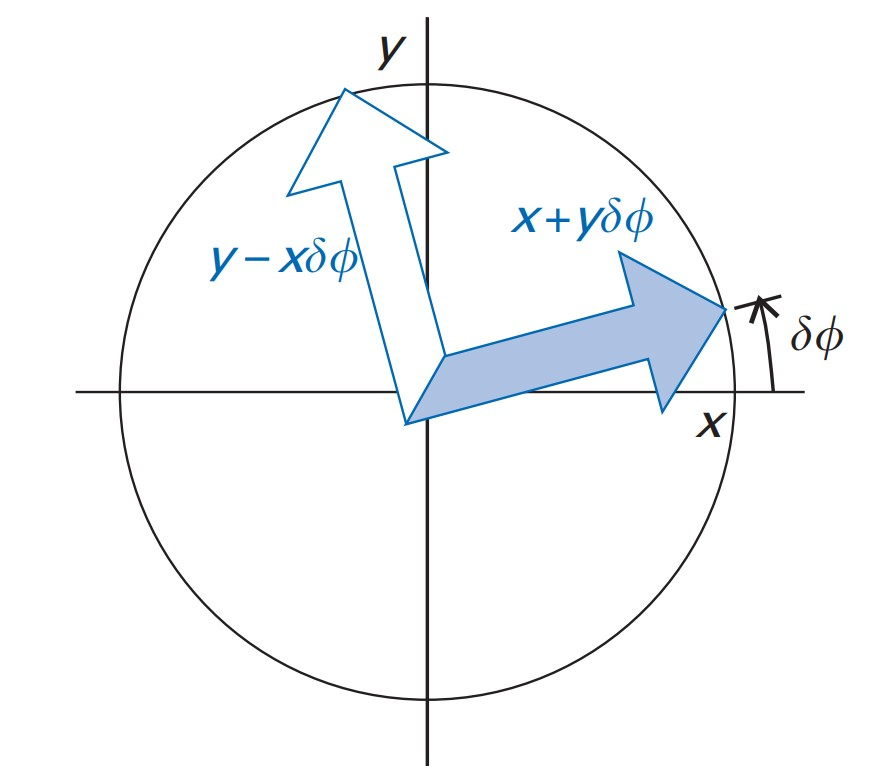
\includegraphics[width=6cm]{c2rot}
	\centering
	\caption{The effect of $C_{\delta\phi}$ on the basis of $(x,y)$.}
	\label{fig:c2rot}
\end{figure}
We have effectively expressed the classical operation $C_{\delta\phi}$ in the language of quantum mechanics, and we can call $\hat{l}_z$ the quantum mechanical generator of rotations about the $z$-axis\footnote{The classical $\hat{l}_{z,\text{class}}$ does away with the $\hbar$, \ie is just $\hat{l}_{z,\text{quant}}/\hbar$}\par
Now moving onto $R_3$, a sequential $x$ and $y$ rotation gives
\begin{equation}
\begin{aligned}
	C_{\delta\beta}^{(y)}C_{\delta\alpha}^{(x)}&=\lf(1-\frac{i}{\hbar}\delta\beta\hat{l}_y+\dots \rt)\lf(1-\frac{i}{\hbar}\delta\alpha\hat{l}_x+\dots \rt)\\
	&=1-\frac{i}{\hbar}(\delta\beta\hat{l}_y+\delta\alpha\hat{l}_x)+\lf(\frac{i}{\hbar} \rt)^2\delta\beta\delta\alpha\hat{l}_x\hat{l}_y+\dots
\end{aligned}
\end{equation}
but a sequential $y$ and $x$ rotation gives
\begin{equation}
\begin{aligned}
	C_{\delta\alpha}^{(x)}C_{\delta\beta}^{(y)}&=\lf(1-\frac{i}{\hbar}\delta\alpha\hat{l}_x+\dots \rt)\lf(1-\frac{i}{\hbar}\delta\beta\hat{l}_y+\dots \rt)\\
	&=1-\frac{i}{\hbar}(\delta\beta\hat{l}_y+\delta\alpha\hat{l}_x)+\lf(\frac{i}{\hbar} \rt)^2\delta\beta\delta\alpha\hat{l}_y\hat{l}_x+\dots
\end{aligned}
\end{equation}
so we can see that the difference between these two to the second order is 
\begin{equation}
	C_{\delta\beta}^{(y)}C_{\delta\alpha}^{(x)}-C_{\delta\alpha}^{(x)}C_{\delta\beta}^{(y)}=\lf(\frac{i}{\hbar} \rt)^2\delta\alpha\delta\beta(\hat{l}_y\hat{l}_x-\hat{l}_x\hat{l}_y)=\frac{i}{\hbar}\delta\alpha\delta\beta\hat{l}_z
\end{equation}
\begin{figure}[H]
	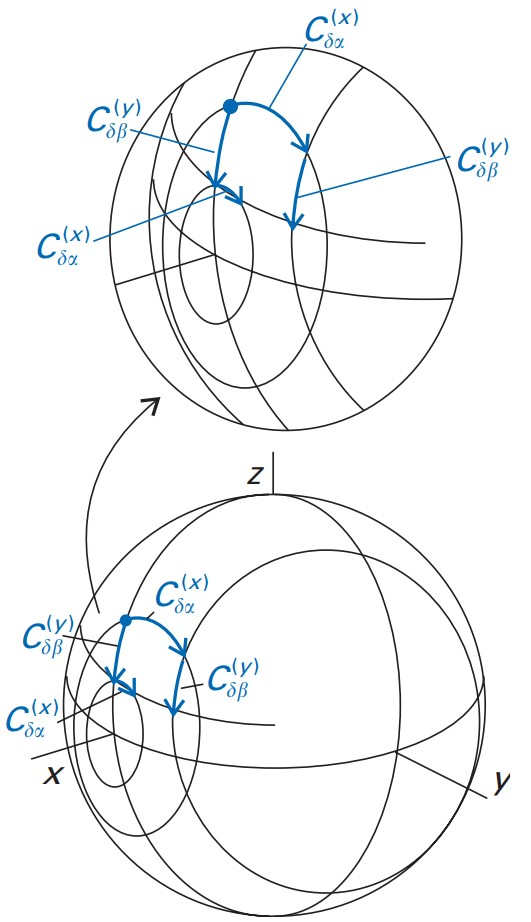
\includegraphics[width=6cm]{r3rot}
	\centering
	\caption{The difference between the two composite rotations, we can see the commutation relations graphically.}
	\label{fig:r3rot}
\end{figure}
\paragraph{The representation of the full rotation group}
The spherical harmonics $Y_{l,m_l}$ for a given $l$ transform into linear combinations of one another under a rotation, for example, the $p$-orbitals rotate into one another but not into $d$-orbitals. This is an examplification of \cref{degeneigen}, which says degenerate eigenfunctions can be related by symmetry operations.\par
Therefore, the functions $Y_{l,l},Y_{l,l-1},\dots,Y_{l,-l}$ form a basis for a $(2l+1)$-dimensional representation of the gruop. As they are orthonormal to each other, the representation is irreducible. The spherical harmonic has the form $Y_{l,m_l}=P_l^{m_l}(\cos\theta)\exp(im_l\phi) $ (\cref{sphericalharmonics}) so a rotation by $\alpha$ about the $z$-axis gives $P(\cos\theta)\exp(im_l(\phi-\alpha)) $, extending this to the entire basis we have
\begin{equation}
\begin{aligned}
	&C_{\alpha}^{(z)}(Y_{l,l},Y_{l,l-1},\dots,Y_{l,-l})\\
	=&P(\cos\theta)\lf\{\exp[il(\phi-\alpha)],\exp[i(l-1)(\phi-\alpha)],\dots,\exp[-il(\phi-\alpha)] \rt\}\\
	=&(Y_{l,l},Y_{l,l-1},\dots,Y_{l,-l})
	\begin{bmatrix}
		e^{-il\alpha} & 0 & 0 & \cdots & 0\\
		0 & e^{-i(l-1)\alpha} & 0 & \cdots & 0\\
		0 & 0 & \ddots &  & 0\\
		\vdots & \vdots &  & \ddots & \vdots \\
		0&0&\cdots&\cdots&e^{il\alpha}
	\end{bmatrix}
\end{aligned}
\end{equation}
We have identified the matrix representative of the rotation in this basis. The character of rotation is then 
\begin{equation}
\begin{aligned}
	\chi(C_{\alpha})&=e^{-il\alpha}+e^{-i(l-1)\alpha}+\dots+e^{il\alpha}\\
	&=\frac{e^{-il\alpha}[e^{i(2l+1)\alpha}-1] }{e^{i\alpha}-1}\\
	&=\frac{\sin(l+\tfrac{1}{2})\alpha}{\sin\tfrac{1}{2}\alpha}
\end{aligned}
\end{equation}
In the limit of $\alpha\rightarrow0$ (infinitesimal rotation as a symmetry operation) we get the character as $2l+1$ so we recover the fact that levels with quantum number $l$ are $(2l+1)$-fold degenerate in a spherical system.
\subsection{Group theory and angular momenta}
In the last section we saw that a quantum rigid rotor belong to the full rotation group. Now suppose there are two rotors with $j_1$ and $j_2$, belonging the irreps $\Gamma^{(j_1)}$ and $\Gamma^{(j_2)} $ with basis functions $f_{mj1}^{(j_1)} $ and $f_{mj2}^{(j_2)} $ respectively.\par
From \cref{decompdirect} we know that the bases for $\Gamma^{(j_1)}\otimes \Gamma^{(j_2)}$ are $f_{mj1}^{(j_1)}f_{mj2}^{(j_2)}$, subject to further reduction, we can write
\begin{equation}
	\Gamma^{(j_1)}\otimes \Gamma^{(j_2)}=\sum_ja_j\Gamma^{(j)}
\end{equation}
The character of rotation the system, when viewed through the decoupled picture, is 
\begin{equation}
	\chi(C_{\alpha})=\chi^{(j_1)}(C_{\alpha})\chi^{(j_2)}(C_{\alpha})=\sum_{m_{j1}=-j_1}^{j_1}\sum_{m_{j2}=-j_2}^{j_2}e^{i(m_{j1}+m_{j2})\alpha}
\end{equation}
As it contains repeated exponentials, we hope to write this in the form of
\begin{equation}
	\chi(C_{\alpha})=\sum_j\sum_{m_j}e^{im_j\alpha}
\end{equation}
which physically represents the coupled picture. To show this is possible, we realise that, purely from the mathematical form, $|m_{j1}+m_{j2}|\leq j_1+j_2$, so $|m_j|\leq j_1+j_2$ and $j\leq j_1+j_2$. Therefore $a_j=0$ for $j>j_1+j_2$. The maximum $m_j$ can only be created in one way, when $m_{j1}=j_1$ and $m_{j2}=j_2$, so $a_{j1+j2}=1$. For $m_j=j_1+j_2-1$, there are two ways to create it but one is already accounted for by the representation with $j=j_1+j_2$, so $a_{j1+j2-1}=1$, and so on. We now have the series 
\begin{equation}
	\Gamma^{(j_1)}\otimes\Gamma^{(j_2)}=\Gamma^{(j_1+j_2)}\oplus\Gamma^{(j_1+j_2-1)}\oplus\dots
\end{equation}
to terminate, we assume for a moment that $j_1>j_2$, noting that $\Gamma^{(j_i)} $ is $(2j_i+1)$-fold degenerate, so $\Gamma^{(j_1)}\otimes \Gamma^{(j_2)}$ is $(2j_1+1)(2j_2+1)$-fold degenerate, if the series terminate at $j_1-j_2$, the degeneracy on the right hand side equals the left:
\begin{equation}
\begin{aligned}
	\text{RHS}&=2[(j_1+j_2)+(j_1+j_2-1)+\dots+(j_1+j_2-2j_2)] +2j_2+1\\
	&=4j_1j_2+2j_1+2j_2+1\\
	&=\text{LHS}
\end{aligned}
\end{equation}
 This argument is exactly analogous to that given in \cref{perm_totmom}. We can write 
\begin{equation}
	\chi(C_{\alpha})=\sum_{j=|j_1-j_2|}^{j_1+j_2}\sum_{m_j=-j}^je^{im_j\alpha}=\sum_{j=|j_1-j_2|}^{j_1+j_2}\chi^{(j)}(C_{\alpha})
\end{equation}
This is essentially saying
\begin{equation}
	\Gamma^{(j_1)}\otimes\Gamma^{(j_2)}=\Gamma^{(j_1+j_2)}\oplus\Gamma^{(j_1+j_2-1)}\oplus\dots\oplus\Gamma^{(|j_1-j_2|)}
\end{equation}

\section{Applications}
\subsection{Vanishing integrals}
Consider two functions $f$ and $g$, one antisymmetric and the other symmetric 
about $x=0$. Now consider their integrals on the interval $[-a,+a]$: that of $f$ 
necessarily zero and that of $g$ can only be zero by accident. Now, if we look 
closely at the interval $[-a,+a]$ as an object, it belongs to point group $C_s$: 
identity and mirror plane. Function $f$ can be a basis of the irrep $A''$ because 
$Ef=f,\ \sigma_hf=-f$. Meanwhile, $g$ spans $A'$, the totally symmetric irrep. 
So we generalise:
\begin{lemma}[Vanishing integral]
The integral is necessarily zero if the integrand is a basis for the totally 
symmetric irreducible representation of the group. 
\end{lemma}
We now examine the products between $f$ and $g$:
\begin{enumerate}
	\item $f^2$: $A''\otimes A''=A'$, non-vanishing.
	\item $g^2$: $A'\otimes A'=A'$, non-vanishing.
	\item $fg$: $A''\otimes A'=A''$, vanishing. 
\end{enumerate}
Another way to look at this is that $f$ and $g$ are basis functions for different 
species therefore they must be orthogonal:
\begin{lemma}[Generalised vanishing integral]
If $f_i^{(\ell)}$ is the $i$-th member of a basis that spans the irrep of species 
$\Gamma^{(\ell)}$ of a group, and $f_j^{(\ell)}$ is the $j$-th member of a basis 
that spans the irrep of species $\Gamma^{(\ell)}$ of the same group, then for 
a symmetric range of integration
\begin{equation}
\int f_i^{(\ell)*}f_j^{(\ell')}\dif\tau\propto\delta_{\ell\ell'}\delta_{ij}
\end{equation}
\end{lemma}
We now are in a position to state the most important result so far
\begin{thrm}[Zero integrals]
\label{zerointegral}
An integral $\int f^{(\ell)*}f^{(\ell')}\dif\tau$ over a symmetric range is 
necessarily zero unless the integrand is a basis for the totally symmetric 
irreducible representation of the group which will be the case only if 
$\Gamma^{(\ell)}=\Gamma^{(\ell')}$. 
\end{thrm}
This can be extended to integrals of the form
\begin{equation}
I=\int f^{(\ell)*}f^{(\ell')}f^{(\ell'')}\dif\tau
\end{equation}
where the integral is necessarily zero unless the integrand is a basis for the 
totally symmetric irrep: we take $\Gamma^{(\ell)}\times\Gamma^{(\ell')}$ and 
expand out, then we take each $\Gamma^{(k)}$ in the expansion and form direct 
products $\Gamma^{(k)}\times\Gamma^{(\ell'')}$. If the tot. sym. irrep does not 
occur in the final expansion, then the integral is necessarily zero. \par
An important application of this would be determining whether a matrix element such as $H_{ij}=\lgl \psi_i |\psi_j  \rgl $ is zero. \par
In the case of the Hamiltonian, we know it is rotationally invariant \ie it belongs to the totally symmetric irrep, so all we really need to determining is whether $\psi_i$ and $\psi_j$ belong to the same irrep. \par
Another, more general example is in the case of the \emph{dipole moment operators}:\par
In a $C_{4v}$ (SF$_5$Cl say) molecule, do the integrals $\lgl d_{xy}|z |d_{x^2-y^2}  \rgl $ and $\lgl d_{xy}|l_z |d_{x^2-y^2}  \rgl $ vanish?\\
The objects span the following irreps:
\begin{center}
	\begin{tabular}{c|c}
		Object & Irrep\\
		\hline
		$d_{xy}$ & B$_2$\\
		$d_{x^2-y^2}$ & B$_1$\\
		$z$ & A$_1$\\
		$l_z$ & A$_2$
	\end{tabular}
\end{center}
Since
\begin{equation}
\begin{aligned}
&B_2\otimes A_1\otimes B_1=B_2\otimes B_1\neq A_1\\
&B_2\otimes A_2\otimes B_1=B_2\otimes B_2=A_1
\end{aligned}
\end{equation}
the former must vanish and the latter not necessarily.
\subsection{Degeneracy}
The Hamiltonian of a system must be invariant under every operation of the point 
group of the system:
\begin{equation}
RH\equiv H.
\end{equation}
A mathematical way of reasoning is that, because $H\equiv T+V$, which, take the one-dimensional harmonic oscillator for example, depends on $\diff[2]{}/{x}$ and 
$x^2$ respectively, and as such it's invariant under replacement of $x$ by $-x$, 
so the Hamiltonian spans the tot. sym. irrep of $C_s$. \par
Because $H$ is invariant under a similarity transformation of the group, \ie 
change of basis, or symmetry operation, we can write
\begin{equation}
RHR^{-1}=H.
\end{equation}
Right multiplication with $R$ gives $RH=HR$, so we can conclude that symmetry 
operations must commute with the Hamiltonian. We then introduce
\begin{thrm}[Degenerate eigenfunctions]
\label{degeneigen}
Eigenfunctions that are related by symmetry transformations of the system are degenerate, and \emph{vice versa}. 
\end{thrm}
\begin{proof}
Consider $H\psi_i=E\psi_i$. Right multiplying by $R$ gives
\begin{equation}
\begin{aligned}
RH\psi_i&=ER\psi_i\\
RH(R^{-1}R)\psi_i&=ER\psi_i\\
HR\psi_i&=ER\psi_i.
\end{aligned}
\end{equation}
Therefore, $\psi_i$ and $R\psi_i$ are degenerate.
\end{proof}
So how to determine the maximum degree of degeneracy? We recall that the 
projection operator $P_{ij}$ can give us all members of a basis set, and that it 
is formed by a linear combination of group operations, so it necessarily commutes 
with the Hamiltonian, therefore, for an irrep of dimension $d$, 
\begin{equation}
P_{ij}H\psi_j=HP_{ij}\psi_j=H\psi_i=P_{ij}E\psi_j=E\psi_i.
\end{equation}
In the same manner we can generate all $d$ members this way and they are all going 
to be degenerate, so
\begin{thrm}[Degree of degeneracy]
The degree of degeneracy of a set of functions is equal to the dimension of the 
irreducible representation they span, \ie
\begin{equation}
D=\chi(E).
\end{equation}
\end{thrm}
\subsection{Chemical bonding}
To find out which orbitals participate in bonding in a molecule, first find an appropriate basis and 
construct a reducible representation of the point group the molecule belongs to, 
and reduce it. It's that simple. We give a few examples. \par
\textbf{$\sigma$ bonding in $D_{3h}$}\\
For a choice of basis along the three bonds, we construct the character table
\begin{center}
\begin{tabular}{c|cccccc}
$D_{3h}$ & E & 2C$_3$ & 3C$_2$ & $\sigma_h$ & 2S$_3$ & 3$\sigma_v$\\
\hline
$\Gamma_1$ & $3$ & $0$ & $1$ & $3$ & $0$ & $1$
\end{tabular}
\end{center}
Reducing it with the help of $D_{3h}$ charater table, we get, for example
\begin{equation}
a(A_1')=\frac{1}{12}(3\times1+0+1\times3+3\times1+0+1\times3)=1
\end{equation}
etc., we get 
\begin{equation}
\Gamma_1=A_1'\oplus E'
\end{equation}
$A_1'$ includes $x^2+y^2$ and $z^2$, which means either the spherically symmetrical $s$ orbital or the $d_{z^2}$ orbital is involved. Same for $E'$, which either involves $p_x$ \textit{and} $p_y$ together or $d_{x^2-y^2}$ \textit{and} $d_{xy}$ together. We know the energy levels of these orbitals and therefore we can say that $s$, $p_x$ and $p_y$, \ie an $sp^2$ set, is involved in bonding.\par
\textbf{$\pi$ bonding in $D_{3h}$}\\
The basis vectors relevant for $\pi$ bonding are a set of three `out-of-plane' vectors forming the reducible representation $\Gamma_2$ and a set of three `in-plane' vectors forming $\Gamma_3$. The characters and reduction is as follows:
\begin{center}
\begin{tabular}{c|cccccc|c}
$D_{3h}$ & E & 2C$_3$ & 3C$_2$ & $\sigma_h$ & 2S$_3$ & 3$\sigma_v$ & irrep\\
\hline
$\Gamma_2$ & $3$ & $0$ & $-1$ & $-3$ & $0$ & $1$ &$A_2''\oplus E''$\\
$\Gamma_3$ & $3$ & $0$ & $-1$ & $3$ & $0$ & $-1$ &$A_2'\oplus E'$
\end{tabular}
\end{center}
Referring to the character table, we can see $\Gamma_2$ corresponds to the orbitals of $p_z,\ (d_{xz},\ d_{yz})$ together 
and $\Gamma_3$ corresponds to either $(p_x,\ p_y)$ or $(d_{x^2-y^2},\ d_{xy})$ together. \hl{what does this really mean? without a priori input how do we know to ignore the d AOs?}
\subsection{LCAOs}
Linear combinations of atomic orbital is a way to form a molecular orbital from a chosen set of basis functions. The symmetry of the LCAO must be the same as the basis functions, and that's where group theory can help us. We use the aromatic cycloproanium ion as an example.\par
\textbf{Cyclopropanium ion - $D_{3h}$}\\
We choose the $p_z$ atomic orbitals of the carbon atoms as the basis functions and since they have exactly the same directional properties as the out-of-plane vectors, the reduction is just $A_2''+E''$ again. 
So we know that the $\pi$ molecular orbitals include a doubly degenerate pair and one singly degenerate orbital. This is as far as group theory can take us. The relative energies of the orbitals can be supplied by the Huckel theory, which tells us that the energies of the orbitals are $(\alpha+2\beta),\ (\alpha-\beta),\ (\alpha-\beta)$.\par
\textbf{Cyclobutadiene - $D_{4h}$}\\
Again choosing the $p_z$ AOs, we get the reduction of $E_g+A_{2u}+B_{2u}$. The energies from Huckel theory is $(\alpha+2\beta),\ \alpha,\ \alpha,\ (\alpha-2\beta)$, and we can identify $\alpha$ with the doubly degenerate $E_g$.
\subsection{Molecular orbital correlation diagrams}
\textbf{H$_2$O}\\
The relevant orbitals are 2H $s$ and O $p$ and $s$ orbitals. 
The oxygen $p_{x/y/z}$ orbitals transform as $A_1,\ B_1,\ B_2$ respectively, 
the $s$ orbital is just $A_1$. 
The two hydrogen $s$ orbitals, \textit{together}\footnote{They must transform together since they're in a molecule, similarly, we can only identify \textit{linear combinations} of the two orbitals that transform as a component of the overall symmetry species.}, transform as $A_1\oplus B_1$. 
We can identify the linear combinations that result in the symmetry species easily as 
$(\phi_1\pm\phi_2)/\sqrt{2}$ for $A_1$ and $B_1$ respectively. \par
After identifying the symmetry species, we label them on the energy correlation diagram accordingly, but in small caps, as species for specific molecules are conventionally labelled. Only objects that belong to the same symmetry species will interact, producing a higher energy and a lower energy object, belonging to the same species. However the relative energy cannot be predicted by group theory as usual. 
\begin{figure}[H]
	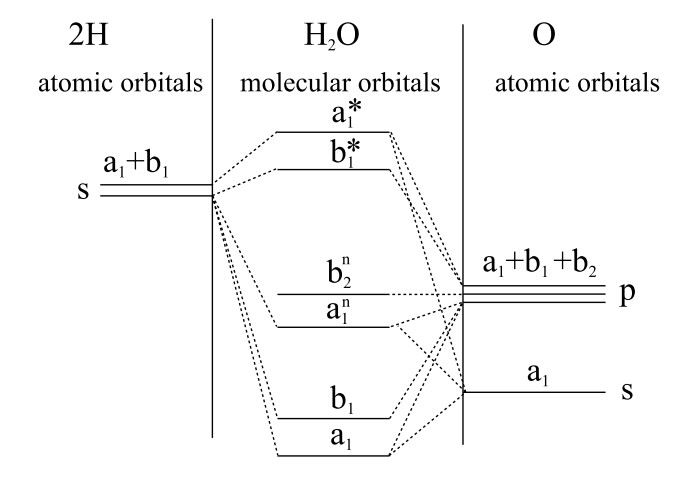
\includegraphics[width=10cm]{h2o_corr}
	\centering
	\caption{The correlation diagram for the water molecule. The two non-bonding orbitals are slightly different in energy, consistent with the photoeletron spectrum.}
	\label{fig:h2o_corr}
\end{figure}
\textbf{[Co(NH$_3$)$_6$]$^{3+}$}\\
The relevant \ie valence orbitals of cobalt are
\begin{center}
	\begin{tabular}{c|c}
	$3d$ ($x^2-y^2$ and $z^2$) & $E_g$\\
	\hline
	$3d$ ($xy,\ xz$ and $yz$) & $T_{2g}$\\
	\hline
	$4s$ & $A_{1g}$\\
	\hline
	$4p$ (all) & $T_{1u}$
	\end{tabular}
\end{center}
And now to reduce the representation formed by the L-M $\sigma$ bonds, we get $A_{1g}\oplus E_g\oplus T_{1u}$. \par
Now let the objects belonging to the same species interact, it's clear that the triply degenerate $3d\ t_{2g}$ orbitals are non-bonding since there are no matching items of the same symmetry. 
\begin{figure}[H]
	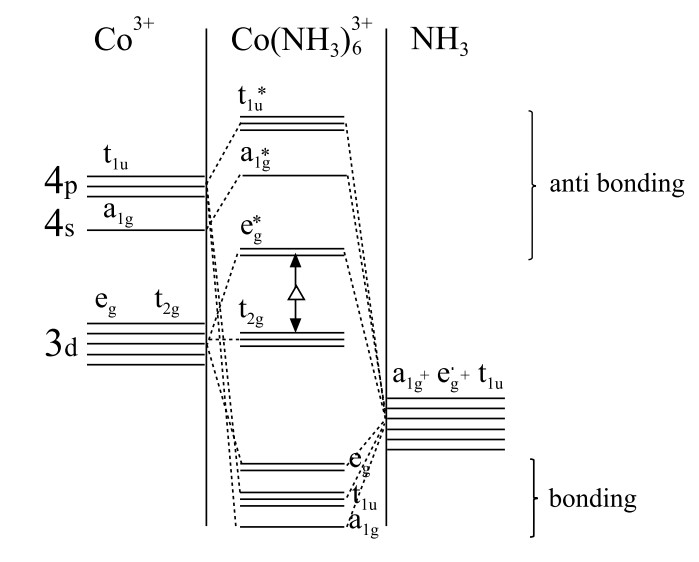
\includegraphics[width=10cm]{cobalt_corr}
	\centering
	\caption{The correlation diagram for the cobalt complex. The gap between $t_{2g}$ and $e_g^*$ is the $\Delta$ from the Ligand Field Theory.}
	\label{fig:cobalt_corr}
\end{figure}
\subsection{Molecular vibrations}
For a molecule with $N$ atoms there are $3N$ coordinates are needed to specify the spatial arrangements of the atoms. Therefore the molecule has $3N$ free variables that can be independently specified\footnote{The strict definition of degree of freedom is the number of variables needed to specify the body's configuration in \emph{phase space}, which will include the momentum \ie velocity vectors, resulting in a total of $6N$ degrees of freedom. Be clear that we're strictly talking about \emph{spatial arrangements} ($\mathbb{R}^3$) here, without considering the velocity vectors, which in this case does not matter all that much (what's knowing the speed of vibration gonna help with anything? The definition is flexible depending on the problem under consideration).}.\par
It is always true that motions of a body can be decomposed into translations, rotations and internal vibrations. For translations only the coordinates of the CoM needs to be specified, which accounts for 3 degrees of freedom, for rotations an axes need to be specified, this will take up 3 more for a non-linear molecule. For a linear molecule however the axes will not contain a component in the bond axis, therefore only 2 degrees are needed. The remaining are the number of vibrational degrees of freedom. 
\begin{thrm}[Number of possible vibrations]
For a non-linear molecule of $N$ atoms there are $3N-6$ possible vibrational modes, and $3N-5$ for a linear molecule.
\end{thrm}
The questions we will be solving is to use group theory to systematically predict the number of infrared-, and Raman-active stretches for a given molecule. The steps are given below:
\begin{enumerate}
	\item Generate a reducible representation using a basis set of 3 principal axes for every atom
	\item Reduce the representation
	\item Remove symmetry species corresponding to translations and rotations
	\item A vibration (one symmetry species, regardless of its degeneracy) is infrared active if it belongs to the same symmetry species as a component of dipole moment ($x,\ y,$ or $z$). It is Raman active if it belongs to the same symmetry species as a component of polarisability (one of the binary products or a combination of them)
\end{enumerate}
\textbf{H$_2$O}\\
The 9-vector basis reduces to $3A_1\oplus A_2\oplus 3B_1\oplus 2B_2$, from which we take out the translations $A_1,\ B_1$ and $B_2$ and rotations $A_2,\ B_1$ and $B_2$. The remaining vibrations are $2A_1\oplus B_1$, which coheres with the 3 degrees of freedom predicted by the rule of thumb. \par
The vibrations belong to symmetry species of both the dipole and polarisability, therefore water has 3 coincident infrared and Raman bands.\par
\textbf{XeF$_4$}\\
The 15-vector basis reduces to $A_{1g}\oplus A_{2g}\oplus B_{1g}\oplus B_{2g}\oplus E_g\oplus 2A_{2u}\oplus B_{2u}\oplus 3E_u $. After removal of translations and rotations we have $A_{1g}\oplus B_{1g}\oplus B_{2g}\oplus A_{2u}\oplus B_{2u}\oplus 2E_u$, a 9-degenerate representation, which coheres, as it should, with the rule of thumb. \par
Of the 9 vibrations, $A_{1g},\ B_{1g}$ and $B_{2g}$ are Raman active; $A_{2u}$ and $2E_u$ are infrared-active. $B_{2u}$ \hl{is active in neither.} Therefore there are 3 each, non-coincident infrared and Raman bands for this molecule. \par
\textbf{NH$_3$}\\
The only thing that's different is that the vectors are not pointing in the principal axes directions. 
This results a little bit of difficulty in the charaters of the rotations. 
The following results are easy to derive:
\begin{prt}[Character of $n$-fold rotation and improper rotation]
\begin{equation}
\begin{aligned}
\chi(C_n)&=1+2\cos{\frac{2\pi}{n}}\\
\chi(S_n)&=-1+\cos{\frac{2\pi}{n}}
\end{aligned}
\end{equation}
\end{prt}
\textbf{H$_3^+$}
The choice of vectors can be made such that three sets of three local axes can be transformed into one another but not mixed \ie they can be reduced separately. \hl{insert image}.
The vibrations are $A_1'+E'$, three vibrations as expected from the rule of thumb. 
\subsection{Particular vibrations}
If we only need to looks at particular vibrations, we can narrow down the choice of basis to just along the vibrations we need, instead of a general $3N$ basis. \par
For example, if we need to figure out how many carbonyl stretches will be present in a molecule, say \textbf{Ni(CO)$_4$} ($D_{4h}$), only a basis of 4 vectors are needed. It should be noted that the vector here represents extension and compression, not physical displacement from the central metal atom, so they can never be transformed into minus themselves. 
In this case the basis of 4 vectors transform as $A_{1g}\oplus B_{1g}\oplus E_u$, so we know there will be 1 infrared band and 2 Raman bands. 
In this way, geometrical isomers can be identified.\hl{fill in more examples when you have the time}\par
Another example is the ethane C-H stretches (or any X-H strecthes in other molecules). Under $D_{2h}$ group operations we get $A_g+B_{1g}+B_{2u}+B_{3u}$.
\subsection{Projection operator method}
The projection operator method can be used to determine the lienar combination of (an arbitrary set of) basis vectors that makes up a symmetry species. Applications include finding the exact vibrations in a vibrational mode, determining the LCAO, determining the functional form of HAOs, and so on. \par
The method of the projection operator is outlined as follows \hl{update and link this to the formal approach}
\begin{enumerate}
	\item Choose an arbitrary basis, reduce it
	\item Choose a `generating vector', usually something easy to work with but it's arbitrary. If degeneracy is present in any of the irreps, orthogonal generating vectors has to be chosen (\emph{e.g.} $E_g$ requires two orthogonal generating vectors whereas $T_g$ requires three)
	\item Use the \emph{extended} character table, contruct the effect of the individual operations on the generating vector
	\item Multiply all the entries with the character of the irrep, sum each row up
	\item Normalise the results
\end{enumerate}
Example: Vibrations of \textbf{BCl$_3$} ($D_{3h}$)\\
\begin{figure}[H]
	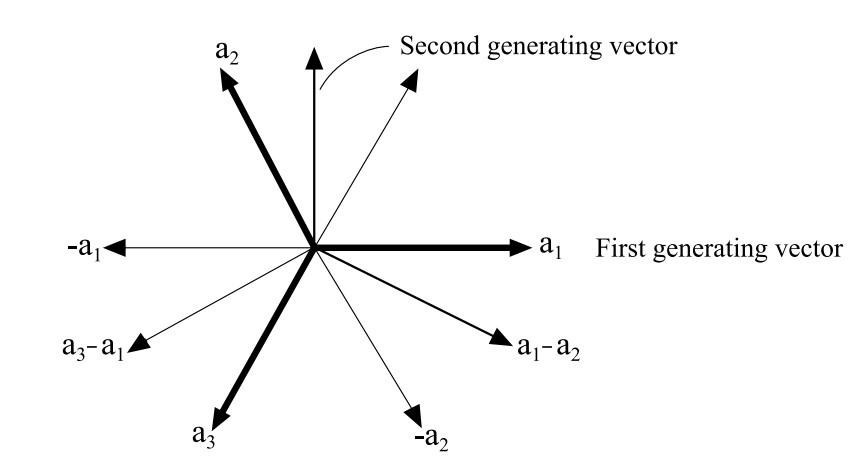
\includegraphics[width=10cm]{bcl3_vec}
	\centering
	\caption{The choice of basis and generating vectors.}
	\label{fig:bcl3_vec}
\end{figure}
\begin{figure}[H]
	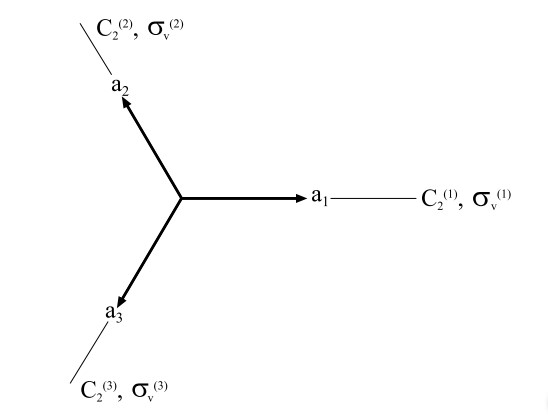
\includegraphics[width=10cm]{bcl3_sym}
	\centering
	\caption{The operations.}
	\label{fig:bcl3_sym}
\end{figure}
\textbf{Step 1:} The three-arrow basis along the bonds reduces to $A_1'+E'$.\\
\textbf{Step 2:} For the $A_1'$ mode we use $a_1$ as the generating vector, and for the $E'$ mode we use $a_1$ and one vector orthogonal to it, $a_2-a_3$\footnote{The magnitude doesn't matter.}. \\
\textbf{Step 3:} Using the extended charater table, we have
\begin{center}
	\begin{tabular}{c|cccccccccccc}
$D_{3h}$ & $E$ &$C_3$&$C_3^2$&$C_2(1)$&$C_2(2)$&$C_2(3)$&$\sigma_h$&$S_3$&$S_3^5$&$\sigma_v(1)$&$\sigma_v(2)$&$\sigma_v(3)$\\
\hline
$A_1'$ ($a_1$)&$a_1$&$a_2$&$a_3$&$a_1$&$a_3$&$a_2$&$a_1$&$a_2$&$a_3$&$a_1$&$a_3$&$a_2$ \\
$E'$ ($a_1$)&\multicolumn{5}{l}{Same as above}\\
$E'$ ($a_2-a_3$)&\dots
	\end{tabular}
\end{center}
\textbf{Step 4 and 5:} Now multiplying with the character and summing the rows, we get the normalised results
\begin{center}
	\begin{tabular}{c|c}
	Mode & Orthonormal basis\\
	\hline
	$A_1'$ & $\frac{1}{\sqrt{3}}(a_1+a_2+a_3)$\\
	$E'(x)$ & $\frac{1}{\sqrt{6}}(2a_1-a_2-a_3) $\\
	$E'(y)$ & $\frac{1}{\sqrt{2}}(a_2-a_3) $
	\end{tabular}
\end{center}
It is easy to verify that the basis is orthonormal: this means that all three bonds contribute equally as they must be due to indistinguishability. \par
The very same approach can be used to find the functional form of the HAOs of boron. We can easily identify the boron $s$ as belonging to $A_1'$, $p_x$ and $p_y$ belonging to $E'$. So we can write
\begin{center}
	\begin{tabular}{c|c}
	Orbital & Orthonormal basis\\
	\hline
	$s$ & $\frac{1}{\sqrt{3}}(a_1+a_2+a_3)$\\
	$p_x$ & $\frac{1}{\sqrt{6}}(2a_1-a_2-a_3) $\\
	$p_y$ & $\frac{1}{\sqrt{2}}(a_2-a_3) $
	\end{tabular}
\end{center}
Rearranging, we have
\begin{center}
	\begin{tabular}{c|c}
	Bond & HAO\\
	\hline
	$a_1$ & $\frac{1}{\sqrt{3}}(s+\sqrt{2}p_x)$\\
	$a_2$ & $\frac{1}{\sqrt{6}}(\sqrt{2}s-p_x+\sqrt{3}p_y) $\\
	$a_3$ & $\frac{1}{\sqrt{6}}(\sqrt{2}s-p_x-\sqrt{3}p_y) $
	\end{tabular}
\end{center}
Again it can be seen that all three orbitals contribute equally to the three HAOs.